\documentclass[11pt,letterpaper]{article}
\usepackage[lmargin=1in,rmargin=1in,tmargin=1in,bmargin=1in]{geometry}
\usepackage{../style/homework}
\usepackage{../style/commands}
\setbool{quotetype}{true} % True: Side; False: Under
\setbool{hideans}{false} % Student: True; Instructor: False

% -------------------
% Content
% -------------------
\begin{document}

\homework{13: Due 11/06}{Teachers open the door, but you must enter by yourself.}{Chinese Proverb}

% Problem 1
\problem{10} Find the inverse of the linear function $\ell(x)= \frac{5}{6} - 8x$. Use this inverse function to solve the equation $\ell(x)= 10$. \pspace

\sol We know that $\ell(x)= \frac{5}{6} - 8x$ is a non-constant linear function (because $m= -8 \neq 0$); therefore, $\ell(x)$ has an inverse. To find the inverse of $\ell(x)= \frac{5}{6} - 8x$, we interchange the `role' of $\ell$ and $x$, and then we solve for $\ell$. The resulting function will be the inverse of $\ell(x)$:
	\[
	\begin{aligned}
	\ell= \frac{5}{6} - 8x \squiggle x&= \frac{5}{6} - 8\ell \\[0.3cm]
	6x&= 5 - 48\ell \\[0.3cm]
	6x - 5&= -48\ell \\[0.3cm]
	\ell&= \dfrac{6x - 5}{-48} \\[0.3cm]
	\ell&= \dfrac{5 - 6x}{48}
	\end{aligned}
	\]
Therefore, $\ell^{-1}(x)= \frac{5 - 6x}{48}$. We can even verify this:
	\[
	\begin{aligned}
	(\ell^{-1} \circ \ell)(x)&= \ell^{-1} \big(\ell(x) \big)= \ell^{-1} \left( \frac{5}{6} - 8x \right)= \dfrac{5 - 6 \cdot \left( \frac{5}{6} - 8x \right)}{48}= \dfrac{5 - 5 + 48x}{48}= \dfrac{48x}{48}= x \\[0.3cm]
	(\ell \circ \ell^{-1})(x)&= \ell \big( \ell^{-1}(x) \big)= \ell \left( \dfrac{5 - 6x}{48}\right)= \dfrac{5}{6} - 8 \left( \dfrac{5 - 6x}{48} \right)= \dfrac{5}{6} - \left( \dfrac{5 - 6x}{6} \right)= \dfrac{5}{6} - \dfrac{5}{6} + x= x
	\end{aligned}
	\]
We can now use $\ell^{-1}$ to solve the equation $\ell(x)= 10$:
	\[
	\begin{gathered}
	\ell(x)= 10 \\[0.3cm]
	\ell^{-1}\big( \ell(x) \big)= \ell^{-1}(10) \\[0.3cm]
	x= \ell^{-1}(10) \\[0.3cm]
	x= \dfrac{5 - 6(10)}{48} \\[0.3cm]
	x= \dfrac{5 - 60}{48} \\[0.3cm]
	x= \dfrac{-54}{48} \\[0.3cm]
	x= -\dfrac{9}{8}
	\end{gathered}
	\]



\newpage



% Problem 2
\problem{10} Explain why the lines $\ell_1(x)= 8x + 3$ and $\ell_2(x)= 9 - 5x$ intersect. Find their point of intersection. \pspace

\sol The slope of the line $\ell_1$ is $m_1= 8$ and the slope of the line $\ell_2$ is $m_2= -5$. Because $m_1= 8 \neq -5= m_2$, the lines cannot be parallel. Therefore, the lines must intersect. If the lines intersect at $(x_0, y_0)$, then we know that $\ell_1(x_0)= y_0= \ell_2(x_0)$. But then\dots
	\[
	\begin{gathered}
	\ell_1(x_0)= \ell_2(x_0) \\[0.3cm]
	8x_3 + 3= 9 - 5x_0 \\[0.3cm]
	13x_0= 6 \\[0.3cm]
	x_0= \dfrac{6}{13}
	\end{gathered}
	\]
But then using this in the first line, we have\dots \pspace
	\[
	\ell_1 \left( \dfrac{6}{13} \right)= 8 \cdot \dfrac{6}{13} + 3= \dfrac{48}{13} + 3= \dfrac{48}{13} + \dfrac{39}{13}= \dfrac{87}{13}
	\] \pspace
Therefore, the lines intersect at the point $\left( \frac{6}{13}, \frac{87}{13} \right) \approx (0.461, 6.692)$. \pspace
	\[
	\fbox{
	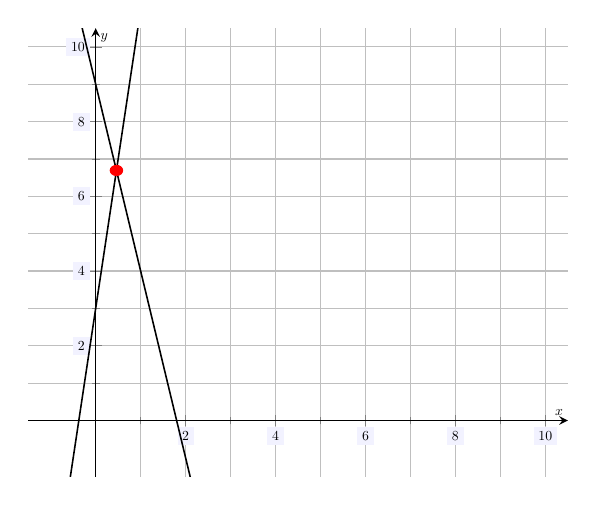
\begin{tikzpicture}[scale=1,every node/.style={scale=0.5}]
	\begin{axis}[
	grid=both,
	axis lines=middle,
	ticklabel style={fill=blue!5!white},
	xmin= -1.5, xmax=10.5,
	ymin= -1.5, ymax=10.5,
	xtick={0,2,4,6,8,10},
	ytick={0,2,4,6,8,10},
	minor tick = {0,1,...,10},
	xlabel=\(x\),ylabel=\(y\),
	]
	\addplot[line width= 0.02cm,samples=2,domain= -1:10.5] ({x},{8*x + 3});
	\addplot[line width= 0.02cm,samples=2,domain= -1:10.5] ({x},{9 - 5*x});
	\draw[draw=none, fill=red,] (6/13,87/13) circle (0.15);
	\end{axis}
	\end{tikzpicture}
	}
	\] 



\newpage

 

% Problem 3
\problem{10} Find the line perpendicular to the line $y= 7 - \frac{2}{3}x$ that contains the $x$-intercept of the line $y= 7x + 3$. \pspace

\sol Because the line $y= 7 - \frac{2}{3}x$ is not horizontal (because the slope is $-\frac{2}{3} \neq 0$), the line in question is not vertical; therefore, the line has the form $y= mx + b$ for some $m, b$. The line is perpendicular to the line $y= 7 - \frac{2}{3}x$. Perpendicular lines have negative reciprocal slopes. The slope of $y= 7 - \frac{2}{3}x$ is $-\frac{2}{3}$. Therefore, our line has slope $m= -\frac{1}{-\frac{2}{3}}= -(-\frac{3}{2})= \frac{3}{2}$. Then we know $y= \frac{3}{2}x + b$. \pspace

The line contains the $x$-intercept of the line $y= 7x + 3$. The $x$-intercept is the point(s) where the curve intersects the $x$-axis, where $y= 0$. But then\dots
	\[
	\begin{gathered}
	0= 7x + 3 \\
	7x= -3 \\
	x= -\dfrac{3}{7}
	\end{gathered}
	\]
Therefore, the $x$-intercept of $y= 7x + 3$ is the point $(-\frac{3}{7}, 0)$. Therefore, the line in question contains the point $(-\frac{3}{7}, 0)$. But then $y= 0$ when $x= -\frac{3}{7}$, so that\dots
	\[
	\begin{gathered}
	y= \frac{3}{2}x + b \\
	0= \frac{3}{2} \cdot -\frac{3}{7} + b \\
	0= -\frac{9}{14} + b \\
	b= \frac{9}{14}
	\end{gathered}
	\]
Therefore, the line is\dots
	\[
	y= \frac{3}{2}\,x + \frac{9}{14}
	\]



\newpage



% Problem 4
\problem{10} Write down an expression that gives the equation for all linear functions passing through the point $(3, 5)$, then use this to find the line that passes through $(3, 5)$ and has $x$-intercept $-6$. \pspace

\sol We know that the graph of a linear function is a line. Given a line with slope $m$ that passes through a point $(x_0, y_0)$, we know that the equation of the line is $y= y_0 + m(x - x_0)$. Because the line contains the point $(3, 5)$, we know that the linear function is $y= 5 + m(x - 3)$. Therefore, every linear function containing the point $(3, 5)$ must have the form $y= m(x - 3) + 5$ for some $m$. \pspace

If the line has $x$-intercept $-6$, then the line contains the point $(-6, 0)$---namely, the $x$-intercept. But then the line contains the point $(3, 5)$ and the point $(-6, 0)$. Therefore, the slope is\dots
	\[
	m= \dfrac{\Delta y}{\Delta x}= \dfrac{5 - 0}{3 - (-6)}= \dfrac{5}{9}
	\]
Therefore, the linear function is\dots
	\[
	\begin{gathered}
	y= m(x - 3) + 5 \\[0.3cm]
	y=  \frac{5}{9} (x - 3) + 5 \\[0.3cm]
	y= \frac{5}{9}\, x - \frac{5}{9} \cdot 3 + 5 \\[0.3cm]
	y= \frac{5}{9}\, x - \frac{5}{3} + 5 \\[0.3cm]
	y= \frac{5}{9}\, x - \frac{5}{3} + \dfrac{15}{3} \\[0.3cm]
	y= \dfrac{5}{9}\,x + \dfrac{10}{3}
	\end{gathered}
	\]


\end{document}